\documentclass{beamer}

\usepackage[french]{babel}
\usepackage[utf8x]{inputenc}
\usepackage{graphicx,hyperref,ru,url}
\usepackage[T1]{fontenc}
%\usepackage{moreverb}
\usepackage{verbatim}


% The title of the presentation:
%  - first a short version which is visible at the bottom of each slide;
%  - second the full title shown on the title slide;
\title[Android Eclipse SDK]{
  Application Android avec Eclipse SDK}

% Optional: a subtitle to be dispalyed on the title slide
\subtitle{Arthur Rogery, Adrien Lamant}

% The author(s) of the presentation:
%  - again first a short version to be displayed at the bottom;
%  - next the full list of authors, which may include contact information;
\author[Arthur Rogery, Adrien Lamant]{
  Arthur Rogery, Adrien Lamant \\\medskip
  {\small \nolinkurl{}{arthurrogery@gmail.com}} \\ 
  {\small \nolinkurl{lamant.adrien@gmail.com}}}

% The institute:
%  - to start the name of the university as displayed on the top of each slide
%    this can be adjusted such that you can also create a Dutch version
%  - next the institute information as displayed on the title slide
\institute[Application Android Eclipse SDK]{
  Licence informatique, Université Montpellier II}

% Add a date and possibly the name of the event to the slides
%  - again first a short version to be shown at the bottom of each slide
%  - second the full date and event name for the title slide
\date[20/11/2014]{}
\begin{document}

\begin{frame}
  \titlepage
\end{frame}

\begin{frame}
  \frametitle{Sommaire}

  \tableofcontents
\end{frame}

% Section titles are shown in at the top of the slides with the current section 
% highlighted. Note that the number of sections determines the size of the top 
% bar, and hence the university name and logo. If you do not add any sections 
% they will not be visible.

% =============== INTRODUCTION ===============

\section{Introduction}

\begin{frame}
  \frametitle{Introduction}
  \begin{enumerate}
    \item Histoire d'Androïd
    \item Introduction à Java/Eclipse
    \item Que sont l'ADT et le SDK ?
  \end{enumerate}
\end{frame}



\begin{frame}
  \frametitle{Introduction - Histoire d'Androïd}
    \begin{figure}
    \centering
    \includegraphics[width=3cm,height=3cm]{android.eps}
    \end{figure}
    \begin{itemize}
        \item Un système d'exploitation mobile multi-plateformes
        \item Open Source de noyau Linux
        \item De la création au rachat par Google
        \item Stratégie de l'OS
    \end{itemize}
\end{frame}



\begin{frame}
  \frametitle{Introduction - Introduction à Java/Eclipse}
   \begin{block}{Java}
    \begin{itemize}
        \item Java,créé en 1995 par James Gosling et Patrick Naughton (Sun Microsystems)
        \item Un langage orienté objet
        \item Résolument "Multi-System"
    \end{itemize}
  \end{block}
  \pause
  \begin{block}{Eclipse, un IDE associé}
    \begin{itemize}
      \item Utilise l'outil JDK (Dev Kit)
      \item Garantit la portabilité des applications
      \item Simplifie la démarche de développement
    \end{itemize}
  \end{block}
\end{frame}



\begin{frame}
  \frametitle{Introduction - ADT et SDK}
    \begin{block}{Qu'est-ce que le bundle ADT}
    \begin{itemize}
        \item Un paquet contenant des fonctionnalités propre à Androïd
        \item Contient des outils spécifiques à Androïd : compileur, débuggeur, packageur...
    \end{itemize}
  \end{block}
  \pause
  \begin{block}{Le Dev Kit SDK}
    \begin{itemize}
      \item Contient un plugin s'intégrant à Eclipse
      \item Permet l'utilisation d'un émulateur
    \end{itemize}
  \end{block}
\end{frame}



% =============== ENVIRONNEMENT DE DEVELOPPEMENT ===============

\section{Environnement de développement}

\begin{frame}
  \frametitle{Environnement de développement}
  \begin{enumerate}
    \item Eclipse
    \begin{itemize}
        \item Historique et évolutions
        \item Utilisation du logiciel
    \end{itemize}
    \item Ressources
        \begin{itemize}
        \item Src / Res / Gen
        \item Documentation Androïd
    \end{itemize}
  \end{enumerate}
\end{frame}



\begin{frame}
  \frametitle{Eclipse - Historique et évolution}
      \begin{figure}
         \centering
          \includegraphics[width=3cm,height=3cm]{eclipse.eps}
      \end{figure}
    \begin{itemize}
        \item Un IDE polyvalent s'appuyant sur le Java
        \item Multi-langages, multi-OS, multi-plateformes
    \end{itemize}
\end{frame}



\begin{frame}
  \frametitle{Eclipse - Utilisation du logiciel}
    \begin{itemize}
        \item Installation des outils
            \begin{itemize}
             \item JDK (Dev Kit Java)
              \item Bundle ADT et SDK (Dev Kit Androïd)
            \end{itemize}
        \item Configuration des outils
            \begin{itemize}
                \item SDK Manager
                \item AVD Emulator
            \end{itemize}
        \item Création d'un projet
    \end{itemize}
\end{frame}



\begin{frame}
  \frametitle{Ressources - Src / Res / Gen}
    \begin{columns}
            \begin{column}{0.33\textwidth}
                \begin{figure}[t]
                    \centering
                    \includegraphics[width=3.5cm,height=5.5cm]{src.eps}
                        \caption{Src}
                \end{figure}
            \end{column}
            \pause
            \begin{column}{0.33\textwidth}
                \begin{figure}[t]
                    \centering
                        \includegraphics[width=3.5cm,height=55mm]{res.eps}
                        \caption{Res}
                \end{figure}
            \end{column}
            \pause
           \begin{column}{0.33\textwidth}
                \begin{figure}[t]
                    \centering
                        \includegraphics[width=3.5cm,height=5.5cm]{gen.eps}
                        \caption{Gen}
                \end{figure}
            \end{column}
    \end{columns}
\end{frame}



\begin{frame}
  \frametitle{Ressources - Documentation Androïd}
    \begin{itemize}
        \item Un manuel complet
        \item \url{http://developer.android.com/index.html}
        \begin{figure}
                    \centering
                        \includegraphics[width=10cm,height=5.5cm]{Doc.eps}
        \end{figure}
    \end{itemize}
\end{frame}

% =============== INTERFACE GRAPHIQUE ===============

\section{Développement d'une interface graphique}

\begin{frame}
  \frametitle{Développement d'une interface graphique}
  \begin{enumerate}
    \item Notions de base de l'interface graphique
    \item Interface à la souris
    \item Interface en XML
        \begin{itemize}
            \item Les Widgets
            \item Gestion des événements
            \item Les Layout
            \item Implémentation
        \end{itemize}
  \end{enumerate}
\end{frame}



\begin{frame}
  \frametitle{Notions de base de l'interface graphique}
  \begin{itemize}
    \item Layout, forme de l'application : \textit{"Un ensemble de vues"}
     \item View,  \textit{"L'affichage graphique"}
     \item Widgets, \textit{"Les briques de base de l'interface graphique"}
  \end{itemize}
\end{frame}

\begin{frame}
  \frametitle{Interface graphique à la souris}
  \begin{itemize}
    \item Presentation de l'outil
    \item Mise en place de Widget
    \item Traduction par Eclipse en XML
  \end{itemize}
          \begin{figure}
            \centering
                \includegraphics[width=10cm,height=4.5cm]{388764.eps}
        \end{figure}
\end{frame}

\begin{frame}
  \frametitle{Les différents widgets}
  \begin{itemize}
  \item Le Textview / EditText
        \begin{figure}
            \centering
                \includegraphics[width=10cm]{TextView.eps}
        \end{figure}
    \pause
    \item Les EditTexts
        \begin{figure}
            \centering
                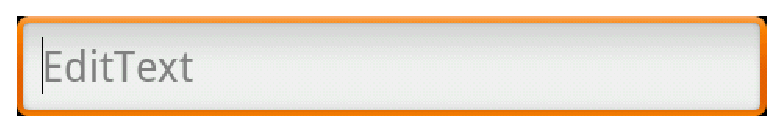
\includegraphics[width=10cm]{TextEdit.eps}
        \end{figure}
  \end{itemize}
\end{frame}



\begin{frame}
  \frametitle{Les différents widgets}
  \begin{itemize}
  \item Les Buttons 
        \begin{figure}
            \centering
                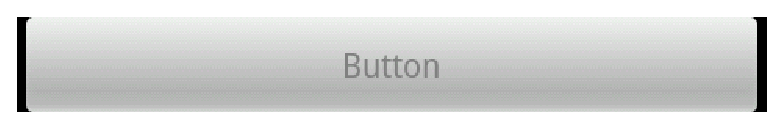
\includegraphics[width=10cm]{Button.eps}
        \end{figure}
        \pause
   \item Les checkBoxs     
        \begin{figure}
            \centering
                \includegraphics[width=10cm]{checkbox.eps}
        \end{figure}
  \end{itemize}
\end{frame}



\begin{frame}
  \frametitle{Les différents widgets}
  \begin{itemize}
    \item Les RadioButtons et RadioGroupes
        \begin{figure}
            \centering
                \includegraphics[width=10cm]{Radio.eps}
        \end{figure}
    \item Un RadioGroup est un layout, mais il n'est utilisé qu'avec des RadioButtons
  \end{itemize}
\end{frame}

\begin{frame}
  \frametitle{Gestion des événements}
    \begin{itemize}
         \item Les listeners
         \item L'interface callbackvoid
         \item Différenciation d'instances
  \end{itemize}
\end{frame}



\begin{frame}
  \frametitle{Les Layouts}
   \begin{enumerate}[1]
        \item Le Principe
        \begin{figure}
            \centering
                \includegraphics[width=5cm,height=5.5cm]{Layout.eps}
        \end{figure}
   \end{enumerate}
\end{frame}



\begin{frame}
  \frametitle{Les Layouts}
   \begin{enumerate}[2]
        \item Les propriétés
            \begin{itemize}
              \item L'orientation
              \begin{itemize}
              \item L’orientation des layouts se fait via la propriété : android:orientation=" orientation”.
les 2 valeurs possibles sont « vertical » et « horizontal ».
            \end{itemize}
        \begin{figure}
          \centering
            \includegraphics[width=5cm,height=4cm]{Horizontal.eps}
        \end{figure}
            \end{itemize}
    \end{enumerate}
\end{frame}



\begin{frame}
 \frametitle{Les Layouts}
    \begin{itemize}
            \item La Taille
                \begin{itemize}
                     \item android:layout\_width et android:layout\_height
                     \item Une taille fixe (en pixels)
                     \item Un fill\_parent
                     \item wrap\_content
                \end{itemize}
    \end{itemize}
\end{frame}



\begin{frame}
    \frametitle{Les Layouts}
        \begin{itemize}
            \item La gravité des éléments
                \begin{itemize}
                    \item Le layout\_gravity
                    \item Le poids grâce à layout\_weight
                \end{itemize}
            \begin{figure}
                \centering
                \includegraphics[width=5cm,height=5cm]{Gravity.eps}
            \end{figure}
    \end{itemize}
\end{frame}

\begin{frame}[containsverbatim]
  \frametitle{Implémentation}
    \begin{itemize}
        \item Implémentation en XML
    \end{itemize}
    \begin{small}
        \begin{verbatim}
          <TextView
          android:layout_width="fill_parent"
          android:layout_height="wrap_content" 
          android:text="Poids : "
          android:textStyle="bold"
          android:textColor="#FF0000"
          android:gravity="center"
   	      \>
        \end{verbatim}
        \end{small}
\end{frame}


\begin{frame}[containsverbatim]
  \frametitle{Implémentation}
    \begin{itemize}
        \item Pour les RadioGroupes
    \end{itemize}
    \begin{tiny}
         \begin{verbatim}
        <RadioGroup
        android:id="@+id/group"
        android:layout_width="wrap_content"
        android:layout_height="wrap_content"
        android:checkedButton="@+id/radio2"
        android:orientation="horizontal"
        >
        <RadioButton 
        android:id="@+id/radio1"
        android:layout_width="wrap_content"
        android:layout_height="wrap_content"
        android:text="Mètre"
     	\>
        <RadioButton 
        android:id="@+id/radio2"
        android:layout_width="wrap_content"
        android:layout_height="wrap_content"
        android:text="Centimètre"
     	\>
        </RadioGroup>
  \end{verbatim}
  \end{tiny}
\end{frame}

% =============== ALTERNATIVE A ECLIPSE ===============



\section{Alternatives à Eclipse}

\begin{frame}
  \frametitle{Alternatives à Eclipse}
  \begin{enumerate}
    \item Android Studio, solution officielle
    \item IDE basés sur Eclipse
    \item Autres IDE
  \end{enumerate}
\end{frame}



\begin{frame}
  \frametitle{Alternatives à Eclipse - Android Studio}
     \begin{itemize}
        \item Un logiciel Google gratuit et OpenSource
        \item Des avantages dans la conception graphique
        \item Facilité de prise en main et d'utilisation
     \end{itemize}
     \begin{figure}[t]
        \centering
         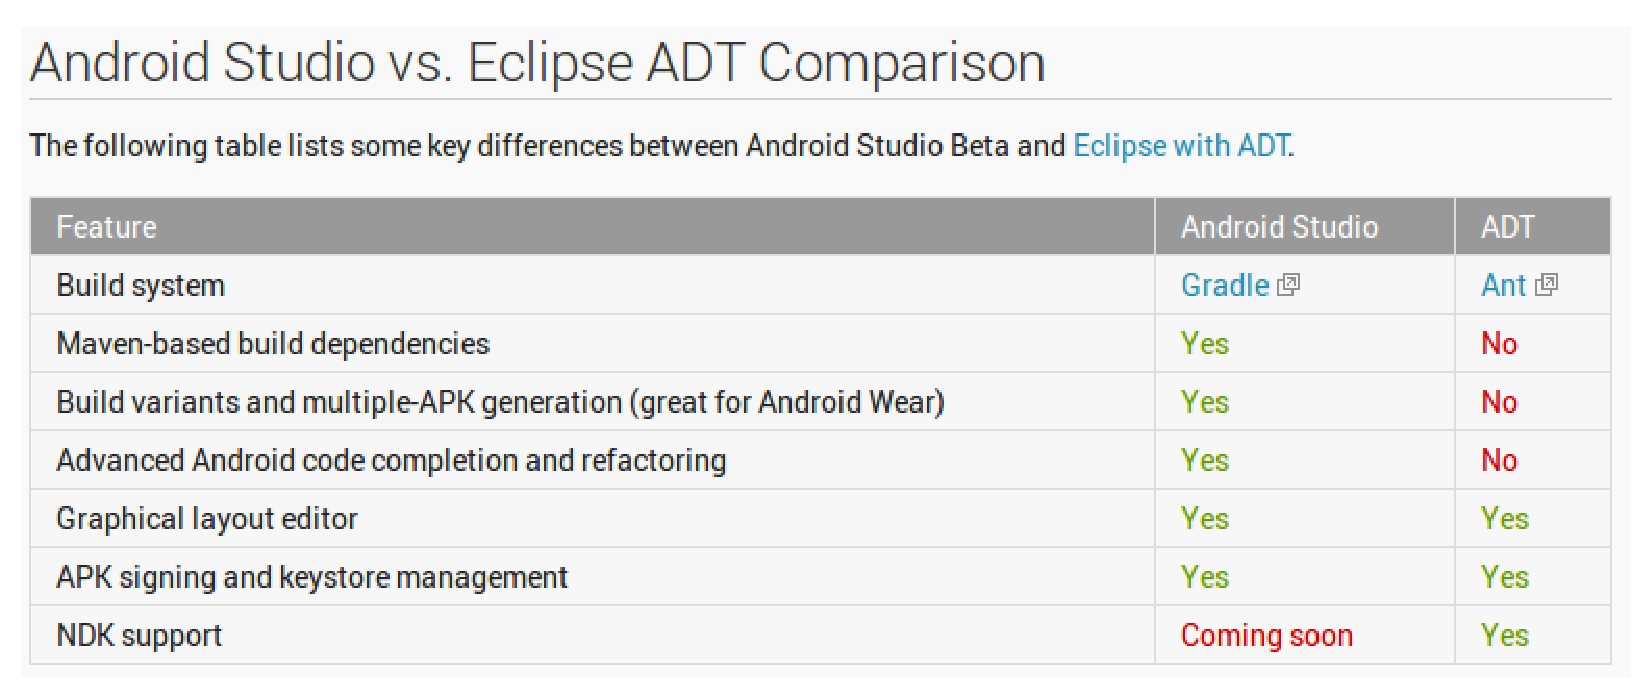
\includegraphics[width=7cm,height=4cm]{difference.eps}
    \end{figure}
\end{frame}



\begin{frame}
  \frametitle{Alternatives à Eclipse}
   \begin{block}{IDE basés sur Eclipse}
    \begin{itemize}
            \item MoSync SDK / MoSync Reload
            \item Titanium Studio
    \end{itemize}
  \end{block}
  \pause
  \begin{block}{Autres IDE}
    \begin{itemize}
        \item IntelliJ IDEA
        \item NBAndroid
    \end{itemize}
  \end{block}
\end{frame}

% =============== CONLUSION ===============

\begin{frame}
  \frametitle{Fin}
\centering Merci de votre attention
\end{frame}

\end{document}